%---------------------------------------------------------------------------------------------------
% Analysis
%---------------------------------------------------------------------------------------------------
\newpage
\chapter{Requirement Analysis}
\label{chap:ReqAnalysis}
 The main requirement of this thesis is to design, and implement an Archive service i.e. back-end web service for the MARS framework. The service's role is to
 archive the MARS resources mentioned in Subsection \ref{subsection:MARSResource} from the Ceph cluster \cite{Ceph} to the 
 NAS\footnote{NAS: Network Attached Storage} Synology drive \cite{Synology}.

 This service targets any user who desires to archive the MARS resources needed for a simulation including the existing simulation results, which would
 be analyzed in the future. The Archive service would expose its API, calling it, one can archive and restore the resources. The exposed
 API is also integrated in the MARS graphical interface (MARS Teaching User Interface). The MARS Teaching API acts as proxy between the users 
 and the MARS back-end Microservices, as it provides some level of abstraction by hiding unnecessary endpoints for the user in the graphical interface.

\newpage
\section{Functional Requirements}
    \label{section:functionalReq}
    This section describes the functional requirements for the Archive service.
    The requirements mentioned here are the expected benchmarks for the designed system which are also depicted in Figure \ref{fig:archiveUseCase}.
    The functional aspects which carves the Archive service are mentioned below.

    \subsection{Archive project resources}
        The designed system should be able to archive the MARS resources from the active system (Ceph cluster at the time of writing) 
        into the Synology \cite{Synology}. The application should
        be able to archive a project even when there all the MARS resources are not present in the project (e.g. no simulation runs have been triggered).
        This should be supported since it could be the case that the user wants to archive only some of the resources. The resources which are to be archived
        are depicted in a tabular format (Table \ref{table: archivedMars}).
        
        \begin{table}[h!]
            \centering
            \begin{tabular}{|p{3cm}|p{12cm}|}
                \hline
                    \textbf{Resource Name}  & \textbf{Description}\\
                \hline
                     Metadata & 
                     This resource stores the metadata (e.g. file id, file name). It gives the system the information about
                     existing files in the system. \\
                \hline
                     Files & 
                     This resource correspond to the models and files which describe a simulation (e.g. wolves and sheep model). \\
                \hline
                     Scenario & 
                     This resource defines the parameters for the model which would be simulated (e.g. simulation run time, number of agents). \\
                \hline
                     Result configurations & 
                     This resource maps which agents in the simulation are present in the simulation run.\\
                \hline
                     Simulation plan & 
                     This resource contains the scenario and the result configuration which can be executed. The simulation plan could be configured to
                     have different scenario and result configuration to produce different kind of output.\\
                \hline
                     Simulation run & 
                     This resource contains the metadata for a simulation results i.e. simulation id, simulation status.\\
                \hline
                     Simulation result & 
                     This resource is the output and contains the results for a single simulation run.\\
                \hline
            \end{tabular}
            \caption{MARS resources which are to be archived}
            \label{table: archivedMars}     
        \end{table} 

        The resources depicted in table (Table \ref{table: archivedMars}) must be archived following the MARS resource hierarchy (Figure \ref{fig:marsDependency}).
        Following the hierarchy, it is arguable why the project is not being archived, despite it being present. Due to the fact that retrieving the project is also 
        desired and it is connected to multiple users which may not exist in the future. To avoid complexity of dealing with many users, the project is
        not archived. 
        \subsubsection{Assurance of correct data being persisted}
            MARS being a Distributed System, Data Coherency (Subsection \ref{subsection: distriChallenges}) 
            is one of the big issue which this thesis faces. As a consequence,
            wrong or unwanted data could be archived. To avoid this the Archive service should include some kind of mechanism that
            could lock the MARS resources during the archive process.
        
        \subsection{Retrieve project resources}    
            The designed software should support the retrieval of the archived projects from the Synology into the active system. The
            system should be able to restore the project given that, the services support the data format which is archived in the Synology.
           
            \begin{figure}[H]
                \centering 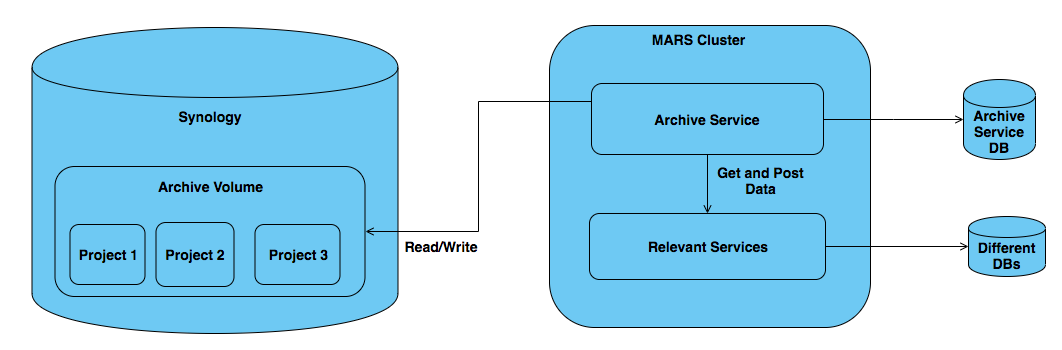
\includegraphics[scale=0.4]{grafiken/synology.png}
                \caption{Archive service's communication structure}
                \label{fig:synology}
            \end{figure}

            Figure \ref{fig:synology} illustrates the communication procedure required to be implemented for the archive and retrieval process. 
            This requirement must be fulfilled to comply with the MARS development standard. As seen, the
            Archive service can read and write directly only to the archive volume in Synology and its own database. The data which is not owned by the archive
            service has to be requested via an API to the relevant service for read/write purposes. The figure generalizes the services it communicates with
            as "Relevant Services" because this diagram only intends to show an abstraction for the communication between them.

        \subsection{Download archived data as a compressed file}
            It is of great importance for a Domain Expert i.e. ecologist to have a graphical interface in hand. In this interface
            it should be possible to navigate to the project of interest and easily download the project as a zip file. There could be cases where the
            MARS system is out of order and the data is required which could then be accessible by anyone with basic knowledge of the system.
        
        \subsection{Design for Failure}   
        Firstly, the Archive service has to communicate with many services in the system, leading the rate of failure being higher
        in comparison to a system which does not depend on other services. A breakdown 
        of one service would cause the whole process of archive/retrieve to stop unexpectedly.  Secondly, it is also possible that a running Archive service be terminated
        due to some unexpected reason. Therefore, fault tolerance mechanism has to be included in the Archive system so that it has a chance of 
        recovery. 

\section{Non functional Requirements}
\label{section:technicalReq}
The requirements specified in this section present us the technical/non-functional aspects of the Archive service. A tabular description 
(Table \ref{table: Technical Requirements}) is presented below.
The detailed description depicts the benchmarks of how the system should be designed to meet the needs for a better sustainable prototype.
The result from this work delivered must comply with the following technical requirements.

    \begin{longtable}{|p{3cm}|p{12cm}|}
            \hline
                \textbf{Requirement}  & \textbf{Description}\\
            \hline
                 Build and deployment & 
                 The service should be deployable in the MARS kubernetus \cite{kubernetes} cluster using the Gitlab pipeline as seen in Figure \ref{fig:CIbuild}
                 which is valid at the time of writing this Thesis. In addition,
                 the build stages for the pipeline also has to be written. \\
            \hline
                Docker containerizing.
                & Choose a suitable Docker container \cite[p.~7 - 8]{Torre2017} for the service. This depends on the type of programming language which 
                the service is being
                written in (e.g. dotnet core, python, java, go).\\
            \hline
                 Scalability & Provide further extensibility option using object orientation so that the service can be scalable.\\
            \hline
                 Robustness & The system should be tested against multiple cases to ensure correct functionality of the service using unit tests and
                 integration tests.\\    
            \hline
                 Performance & The duration of the archive and retrieve process should be measurable. So that a close watch on the performance of the system is 
                 possible. \\    
            \hline
                 Usability & The system should be integrated in the MARS UI so that it is easily usable by all end users.\\    
            \hline
                 Connection to Synology & The Archive service should be able to make a connection to the Synology drive and store desired data successfully.\\ 
            \hline
                 Make a Swagger API interface & The Archive service should have a Swagger \cite{swagger} interface available so that other 
                 developers can use the service with ease.\\         
            \hline
                Follow Microservice patterns & The service should follow data sovereignty pattern for Microservices mentioned in 
                (Subsection \ref{subsection:dataSovereignty}).\\ 
            \hline
                Responsiveness & The API should give some kind of feedback to the user never the less if request cannot be made an 
                error message should be returned instead of no result. \\      
            \hline
        \caption{Technical requirements for the Archive service}
        \label{table: Technical Requirements}     
    \end{longtable} 
  
    \begin{figure}[H]
        \centering 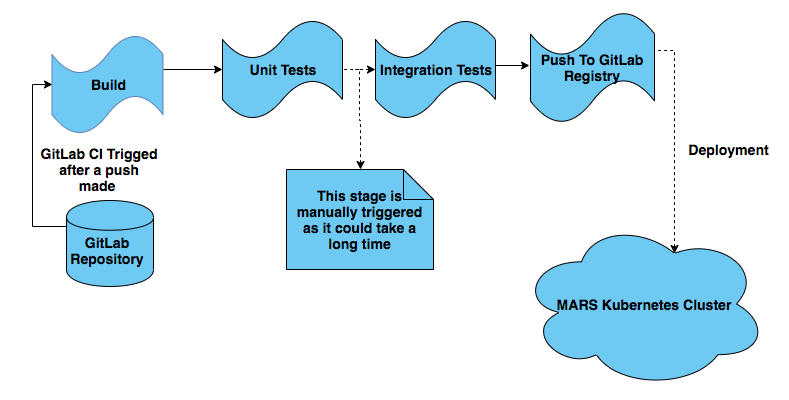
\includegraphics[scale=0.5]{grafiken/CIbuild.png}
        \caption{MARS Continuous Integration Pipeline build}
        \label{fig:CIbuild}
    \end{figure}

    Figure \ref{fig:CIbuild} presents the Continuous Integration system which is being followed at the time of writing this thesis by the MARS developer community.
    The CI\footnote{CI: Continuous Integration} pipeline would be triggered as soon as a new commit is being pushed to the remote 
    GitLab\footnote{https://about.gitlab.com} repository. This would then build the docker image of the service with the new changes. The next step would be to
    run the unit tests written for the service, which is a mandatory step. Lastly, if the pipeline passes, the docker image will be pushed
    to the GitLab registry\footnote{https://about.gitlab.com/2016/05/23/gitlab-container-registry/}. If this is successful then the image can be used in one of 
    the MARS kubernetes cluster i.e. MARS beta, MARS production environments. In addition,
    it can be seen that the integration tests are configured to be an optional test because the integration tests could consume considerably more time and may hinder
    important updates. For this reason, the integration tests are ran manually in the pipeline.
